
\subsection{Basic quantum mechanics}
This part offers a quick introduction to the necessary quantum mechanics for readers who are not familiar with the subject. Quantum mechanics is the framework developed to handle modern physics and is famously somewhat hard to understand intuitively; 
a good baseline understanding is however obtainable with knowledge of linear algebra combined with the postulates of QM. But to understand the contents of this project it should be enough with linear algebra and some physical intrepretation. The section focuses mostly on familiarising the reader with the notation used in quantum mechanics and some fundamental ideas. I suggest chapters 1  and 2 of \cite{Sakurai} for a more complete introduction.


\subsubsection{Quantum states and Dirac notation}
First, let us define what is meant by the term \textbf{state}. In classical physics, a state is defined by the position and momentum of all its constituents. An example is a system of $N$ particles, the state of which would be given by $\{ (\vec{x}, \vec{p})_i \}_{i=1}^N$, where $\vec{x},\vec{p} \in \mathbb{R}^3$ are the position and momentum in 3 dimensions. In Quantum Mechanics (QM) it is more subtle than this since exact information of the system cannot be obtained in the same way. A state is represented by a normalized vector in a \textbf{Hilbert space}, $\mathcal{H}$, a complex inner product space. For $u,v \in \mathcal{H}$ the inner product has the following properties:
\begin{enumerate}
\item  The inner product is conjugate symmetric, $$\inp{u}{v} = \overline{\inp{v}{u}} \in \mathbb{C}$$
\item The inner product is linear in the second argument, for constants $a,b\in \mathbb{C}$, $$\inp{u}{av_1 + bv_2} = a\inp{u}{v_1} + b\inp{u}{v_2}$$
\item The inner product is positive definite, $$\inp{u}{u} = 0 \iff u = 0$$
\end{enumerate}
These properties can be combined to find some other useful facts. Combining the 1st and 2nd property, one obtains

\begin{equation}
\inp{au_1 + bu_2}{v} = \overline{\inp{v}{au_1 + bu_2}} = a^{*}\overline{\inp{v}{u_1}} + b^{*}\overline{\inp{v}{u_2}} =   a^{*}\inp{u_1}{v} + b^{*}\inp{u_2}{v}
\end{equation} 
the inner product is anti-linear in the second term. The 1st and 3rd property yield
\begin{equation}
\inp{u}{u} = \overline{\inp{u}{u}} \implies \text{Im}(\inp{u}{u}) = 0,
\end{equation}
or in words, the inner product of two identical vectors is a real number.

A quantum state is then represented by a normalized vector $v$, $\inp{v}{v} = 1$, in a Hilbert space $\mathcal{H}$. Now a property of vector spaces is that any vector can be multiplied by a matrix, and the resulting vector will be a new vector in the same vector space. This is what is meant when a quantum state is \textbf{acted} upon. For a matrix $A$, we have that 
\begin{equation}
\mathcal{H} \ni v  \xrightarrow{A} Av = v' \in \mathcal{H}.
\end{equation}
That is, acting on a state alters it in various ways. Now let us go from this linear algebra notation to the Dirac notation commonly used in quantum mechanics, also known as bra-ket notation.
Vectors are replaced by \textbf{kets},$\ket{}$, or \textbf{bras},$\bra{}$, $$v \mapsto \ket{\psi}$$
$$v^\dagger \mapsto \bra{\psi}$$
and matrices are replaced by linear operators
$$A \mapsto \hat{A}.$$
The same rules apply to these as for the usual vectors.
The labels inside the brackets do not in themselves have any meanings and are in some sense only that, labels, but more often than not it is used to represent some property of the state. With this notation the inner product between to states $\ket{\psi},\ket{\varphi}$ is written and defined as
\begin{equation}
\bra{\psi}\ket{\varphi} = a_1^{*}b_1 + a_2^{*}b_2 + \dots + a_n^{*}b_n = \begin{pmatrix} a_1^{*} & a_2^{*} & \dots & a_n^{*}\end{pmatrix} \begin{pmatrix} b_1 \\ b_2 \\ \vdots \\ b_n\end{pmatrix}.
\end{equation}
From the properties defined earlier the relations $(\ket{\psi})^\dagger = \bra{\psi}$ and $ (\bra{\psi}\ket{\varphi})^\dagger = \bra{\varphi}\ket{\psi}$, suggests another way to define the states simply as
\begin{equation}
\ket{\psi} = \begin{pmatrix}
a_1 \\ a_2 \\ \vdots \\ a_n
\end{pmatrix},\;
\bra{\psi} = (\ket{\psi})^{\dagger} = (a_1^{*}, a_2^{*}, \dots, a_n^{*}),\; a_1,a_2,\dots,a_n \in \mathbb{C},
\end{equation}
which is nothing more than a complex vector. A common way to represent kets is as a linear combination of eigenkets, which corresponds to the set of eigenvectors. Thus, any ket can be written as a linear combination of these kets if they span the Hilbert space
\begin{equation}
\ket{\Psi} = \sum_{\psi} c_{\psi}\ket{\psi}.
\end{equation}
Following are some example calculations to see how to use Dirac-notation. Let us consider what the effect of the Pauli-Z operator of a spin-$\dfrac{1}{2}$ particle is
\begin{enumerate}[label=\textbf{\alph*)}]
\item on the up position $\ket{\psi} = \ket{\downarrow}$

\item on an arbitrary superposition of up and down $\ket{\psi} = \alpha \ket{\uparrow} + \beta\ket{\downarrow}, |\alpha|^2 + |\beta|^2 = 1, \alpha,\beta \in \mathbb{C}$
\end{enumerate}
Let us first show how this would be done using the matrix representation and then using Dirac notation.
Here the kets $\{\ket{\uparrow} \dot{=} \begin{pmatrix}
1 \\ 0
\end{pmatrix}, \, \ket{\downarrow} \dot{=} \begin{pmatrix}
0 \\ 1
\end{pmatrix} \}$ span the Hilbert space of the particle, they also form an orthonormal basis. The Pauli-Z operator in the matrix representation in this basis is $\sigma_z = \begin{pmatrix}
\,1 & 0 \\
0 & -1 \\
\end{pmatrix}$. Then we have that 

\begin{enumerate}[label = \textbf{\alph*)}]
\item We simply write out the matrices and vectors and get that
\begin{equation}
\sigma_z\ket{\psi} \dot{=} \begin{pmatrix}
\,1 & 0 \\
0 & -1 \\
\end{pmatrix}\begin{pmatrix}
0 \\ 1
\end{pmatrix} = \begin{pmatrix}
0 \\ -1
\end{pmatrix} \dot{=} -\ket{\downarrow}
\end{equation}

\item Same as before but with a superposition (linear combination) up and down 
\begin{equation}
\begin{aligned}
\sigma_z\ket{\psi} \; &\dot{=} \;\begin{pmatrix}
\,1 & 0 \\
0 & -1 \\
\end{pmatrix}\left[\alpha\begin{pmatrix}
1 \\ 0
\end{pmatrix} + \beta\begin{pmatrix}
0 \\ 1
\end{pmatrix} \right] \\ &= \begin{pmatrix}
\alpha \\ -\beta
\end{pmatrix}  \\&= \alpha\begin{pmatrix}
1 \\ 0
\end{pmatrix} -\beta\begin{pmatrix}
0 \\ 1
\end{pmatrix} \\&= \;\alpha\ket{\uparrow} - \beta\ket{\downarrow}
\end{aligned}
\end{equation}
\end{enumerate}
The matrix representation works great for small Hilbert spaces since manipulating small matrices by hand is not very time consuming. Consider now the same calculation using Dirac notation, here the inner product will be a key aspect, and making use of the orthonormality of $\ket{\uparrow},\ket{\downarrow}$ it follows that $\bra{\uparrow}\ket{\uparrow} = \bra{\downarrow}\ket{\downarrow} = 1$ and $\bra{\uparrow}\ket{\downarrow} = \bra{\downarrow}\ket{\uparrow} = 0$.
With Dirac notation operators can be expressed as outer products of bras and kets, thus Pauli-Z can be written as $\sigma_z = \ket{\uparrow}\bra{\uparrow} - \ket{\downarrow}\bra{\downarrow}$.

\begin{enumerate}[label=\textbf{\alph*)}]
\item
\begin{equation}
\begin{aligned}
\sigma_z \ket{\psi} &= (\ket{\uparrow}\bra{\uparrow} - \ket{\downarrow}\bra{\downarrow})\ket{\downarrow} \\&= \ket{\uparrow}\underbrace{\bra{\uparrow}\ket{\downarrow}}_{ = 0} - \ket{\downarrow}\underbrace{\bra{\downarrow}\ket{\downarrow}}_{ = 1} \\&= 0\ket{\uparrow} - 1\ket{\downarrow} \\&= -\ket{\downarrow}.
\end{aligned}
\end{equation}
\item 
\begin{equation}
\begin{aligned}
\sigma_z \ket{\psi} &= \left( \ket{\uparrow}\bra{\uparrow} - \ket{\downarrow}\bra{\downarrow} \right) \left(\alpha\ket{\uparrow} + \beta\ket{\downarrow} \right) \\&= 
\alpha\ket{\uparrow}\underbrace{\bra{\uparrow}\ket{\uparrow}}_{ = 1} - \alpha\ket{\downarrow}\underbrace{\bra{\downarrow}\ket{\uparrow}}_{ = 0}
+
\beta\ket{\uparrow}\underbrace{\bra{\uparrow}\ket{\downarrow}}_{ = 0} - \beta\ket{\downarrow}\underbrace{\bra{\downarrow}\ket{\downarrow}}_{ = 1}\\&= \alpha\ket{\uparrow} - \beta\ket{\downarrow}.
\end{aligned}
\end{equation}
\end{enumerate}
Note that the final answer is the same for both cases, but using Dirac notation there is no need to bother with explicit vectors and matrices, that is one of the strong advantages of the Dirac notation. These calculations are quite analogous to how a quantum gate acting on a qubit works which will be discussed further in the background. In Dirac notation any general matrix $A$ can be written as $A = \sum_{ij} A_{ij}\ket{i}\bra{j}$. Measuring a quantum state $\ket{\psi} = \sum_{n}c_n\ket{n},\, c_n\in \mathbb{C}$ collapses it into a single base ket of the measured basis
\begin{equation}
\ket{\psi} \xrightarrow{\text{Measurement}} \ket{n},
\end{equation}
with probability $|c_n|^2$. 



\subsubsection{Time evolution and the Schrödinger equation}
How does the system evolve when time goes from $t_0$ to some later time $t_1 > t_0$. We can write this as an operator equation $U(t_1,t_0)\ket{\psi(t_0)} = \ket{\psi(t_1)}$, where $U$ is called the time evolution operator. To determine the form of $U$ let us state some physically motivated constraints. To preserve probability $U$ must be unitary, $U^\dagger U = UU^\dagger = 1$. The second property that needs to be fulfilled is composition, $U(t_2,t_0) = U(t_2,t_1)U(t_1,t_0)$, which is to say that applying two consecutive time transformations, first between $t_0 \rightarrow t_1$ and then $t_1 \rightarrow t_2$ is equivalent to applying one transformation between $t_0 \rightarrow t_2$. 
Proceeding, let us define how the time evolution operator would act under an infinitesimal change $dt$,
\begin{equation}
U(t+dt, t) = \mathbf{1} - i\,\Omega\,dt
\end{equation}
with $\Omega$ being Hermitian, $\Omega = \Omega^\dagger$. $\Omega$ can be time dependent, and then must be evaluated at $t$. As $dt$ approaches $0$, $U$ reduces to an identity operator, which is appropriate since if zero time passes the quantum state stay  unchanged.
Let us check the two other properties:
\begin{enumerate}
\item Unitarity
\end{enumerate}
\begin{equation}
\begin{aligned}
U(t_0 +dt, t_0)U(t_0 +dt, t_0)^\dagger &= \left( \mathbf{1} - i\,\Omega\,dt \right)\left(\mathbf{1} + i\,\Omega\,dt \right) \\&= \mathbf{1} + i\,\Omega\,dt - i\,\Omega\,dt + \mathcal{O}(dt^2) \\&\simeq \mathbf{1}
\end{aligned}
\end{equation}
\begin{enumerate}[resume]
\item Composition (assuming, $\Omega$ time independent)
\end{enumerate}
\begin{equation}
\begin{aligned}
U(t + dt_1 + dt_2,t + dt_1)U(t+ dt_1,t) &= (\mathbf{1} - i\,\Omega\,dt_2)(\mathbf{1} - i\,\Omega\,dt_1) \\&= \mathbf{1} - i\,\Omega\,dt_1 - i\,\Omega\,dt_2 + \mathcal{O}(dt^2) \\&\simeq \mathbf{1} - i\,\Omega(dt_1 + dt_2) \\&= U(t + dt_1 + dt_2,t).
\end{aligned}
\end{equation}
From the operator $\Omega$ the Hamiltonian, $H$, is defined, $\Omega = \frac{H}{\hbar}$, where $\hbar$ is Planck's constant. Thus the Hamiltonian will always be Hermitian by definition. So for an infinitesimal time shift the operator has the form $U(t + dt, t) = \mathbf{1} - i\,\frac{H}{\hbar} \,dt$.
Time evolution is closely tied to one of Quantum Mechanics postulates, which is that a closed quantum state evolves according to the Schrödinger equation. From the Schrödinger equation it is clear how $\Omega$ is related to the Hamiltonian. It is common to set $\hbar = 1$, so let us do that from now on. Then the Schrödinger equation is given by 
\begin{equation} 
\begin{aligned}
i \pdv{}{t} \ket{\psi(t)} &= \lim_{dt \rightarrow 0} i\left[ \frac{\ket{\psi(t+dt)} - \ket{\psi(t)}}{dt} \right] \\&= \lim_{dt \rightarrow 0} i\left[ \frac{U(t+dt,t) - \mathbf{1}}{dt} \right]\ket{\psi(t)} \\&= \lim_{dt \rightarrow 0} i\left[ \frac{\mathbf{1} - iH\,dt + \mathcal{O}(dt^2) - \mathbf{1}}{dt} \right]\ket{\psi(t)} \\&= \lim_{dt \rightarrow 0} \left[H + \mathcal{O}(dt) \right]\ket{\psi(t)}  = H\ket{\psi(t)}
\end{aligned}
\label{eq:schro}
\end{equation} 
Now it is clear that the time evolution operator is related to the Schrödinger equation, notice that the solution $\ket{\psi(t)}$ can be written in terms of our time evolution operator as
$\ket{\psi(t)} = U(t,t_0)\ket{\psi(t_0)}$. So given an initial condition we have solved the Schrödinger equation if we can determine $U(t,t_0)$.  
To find the time evolution operator for any time $t$, we could successively repeat the infinitesimal operator until the desired time is reached $t_0 \mapsto t_0 + dt \mapsto t_0 + 2\,dt \mapsto \dots \mapsto t - dt \mapsto t$. For the case of a time independent Hamiltonian, $H$, it could be written as
\begin{equation}
\lim_{N \rightarrow \infty} \left(\mathbf{1} - i\,H\frac{(t-t_0)}{N} \right)^N = \exp\left(- i\,H(t-t_0) \right)
\end{equation}
For simplicity let us assume that $t_0 = 0$, then the time evolution operator for a finite time for a time independent Hamiltonian could be written as $U(t,0) = e^{-i\,H\,t}$. If the Hamiltonian has time dependence but it commutes with itself at different times, then an integral can be introduced in the exponential, $U(t,0) = e^{-i\,\int_0^t \,H(t')\, dt'}$, if the Hamiltonian does not commute at different times it becomes a bit more involved and will not be covered here. But the formal solution can be written as $U(t,0) = \mathcal{T}e^{-i\,\int_0^t \,H(t')\, dt'}$, where $\mathcal{T}$ is time-ordering. This is referred to as the dynamical phase and is the most common type of time evolution. In addition to the dynamic phase there exist a geometric phase associated with some quantum systems and was first studied in periodic systems \cite{berry}. This is discussed further in Section 2.2.6.

To conclude, finding the time evolution operator corresponds to finding the solution to the Schrödinger Equation, which governs the time evolution of quantum systems.

\subsection{Quantum computation and quantum information theory}
\subsubsection{The qubit}
A classical bit is a two-state (binary) system, which means it can occupy either one of two states, $0$ or $1$. So with $n$ bits, there are $2^n$ possible states.

The general way to define a qubit would be any two dimensional quantum system, meaning that the Hilbert space is of dimension 2, $\text{dim}(\mathcal{H}) = 2$. Where qubits are on the form given in Equation \ref{eq:qubit}, any normalized superposition (linear combination) of the basis-kets $\ket{0},\ket{1}$.
\begin{equation}
\label{eq:qubit}
\ket{\psi} = \alpha\ket{0} + \beta\ket{1},\,\alpha,\beta \in \mathbb{C},\, |\alpha|^2 + |\beta|^2 = 1.
\end{equation}
Most of the time it is better to work with the abstract concept of qubits without focusing on the physical implementation, however, there are a lot of similarities with spin-$\dfrac{1}{2}$ particles $\{\ket{\downarrow},\ket{\uparrow}\}$ or energy levels in a trapped ion $\{\ket{g},\ket{e}\}$. That is because abstractly those systems can be represented by the exact same mathematical representation in quantum mechanics, they are all 2-dimensional Hilbert spaces. There is no need to limit the physical system to 2-dimensions. Simply choose two appropriate states which form a 2-dimensional subspace in an appropriate basis. The coefficients $\alpha$ and $\beta$ are the probability amplitudes, and tells with what probability one will find either $\ket{0}$ or $\ket{1}$ when measuring. One finds $\ket{0}$ or $\ket{1}$ with probability $|\alpha|^2$ and $|\beta|^2$, respectively.

The consequence of superposition is that the qubit is not limited to just either 0 or 1, but rather any combination of the two. Superposition together with other QM effects is what is used to create classically impossible algorithms \cite{shor,Grover}. The combined state of two qubits $\ket{\psi_1}$ and $\ket{\psi_2}$ is given by 
\begin{equation}
\ket{\psi_1} \otimes \ket{\psi_2} = (\alpha_1\ket{0} + \beta_1\ket{1})\otimes(\alpha_2\ket{0} + \beta_2\ket{1})
\end{equation}
the tensor product is often omitted and one would write $\ket{\psi_1} \otimes \ket{\psi_2} = \ket{\psi_1}\ket{\psi_2} = \ket{\psi_1, \psi_2}$.
So $n$ qubits is often written as $\ket{x}^{\otimes n},\, x \in \{0,1\}$ which is spanned by kets on the form $\ket{x_0x_1x_2...x_n},\, x_i \in \{0,1\}$, representing all possible bit strings of length $n$. However, this project will limited to single qubit(qudit) systems.

\subsubsection{From classical logic gates to quantum gates}
A model used in classical computation is the circuit model, which consists of wires and logic gates. The wires carry the bit information, 0, 1, and the gates apply different operations. A common gate is the ${\tt NOT}$-gate which flips the content of the bit ${\tt NOT}(0) = 1$ and ${\tt NOT}(1) = 0$. Some other common logic gates are shown in Table \ref{tab:gates}, further, in Figure \ref{fig:circ} is an example of a classical circuit converted into an equivalent quantum circuit.  

\begin{table}[h]
    \centering
    \begin{tabular}{|c|c|c|c|c|}
    \hline
    \multicolumn{2}{|c|}{Input} & ${\tt AND}$ & ${\tt XOR}$ & ${\tt OR}$\\
    \hline
    1 & 0 & 0& 0& 0\\
    0 & 1 & 0& 1& 1\\
    1 & 0 & 0& 1& 1\\
    1 & 1 & 1& 0& 1\\
    \hline
    \end{tabular}
    \caption{Some common classical logic gates.}
    \label{tab:gates}
\end{table}


To make logic gates suitable for quantum computation the classical logic gate has to be adjusted. A quantum gate has some desired properties:
\begin{enumerate}
\item Reversibility,
\item Conservation of probability,
\end{enumerate}
it will turn out that these properties have more or less the same consequence. The first property is not achieved by the classical gates. For example, given the output of the ${\tt XOR}$-gate  it is impossible to know the state of the bits that went into the gate. An output of 1 only conveys that one of the inputs were 1, but not which one. Adding another output that simply is one of the inputs can make the gate reversible. In the quantum mechanical context, a quantum logic gate is a quantum operator acting on the state of the qubit. $A\ket{\psi} = \ket{\psi'}$, so the equivalence of the classical reversibility would be the existence of an inverse operator $A^{-1}$ such that the operation could be reversed $A^{-1}\ket{\psi'} = A^{-1}A\ket{\psi} = \mathbf{1}\ket{\psi} = \ket{\psi}$

Conservation of probability does not in itself have any classical analogue due to it being a quantum property. More concretely it means conservation of the inner product. Given the states $U\ket{\psi} = \ket{\psi'}$ and $U\ket{\varphi} = \ket{\varphi'}$, then the inner product of $\ket{\psi}$ and $\ket{\varphi}$ is the same as for $\ket{\psi'}$ and $\ket{\varphi'}$. Thus one can compute
\begin{equation}
\bra{\psi'}\ket{\varphi'} = \bra{\psi}U^\dagger U\ket{\varphi} = \bra{\psi}\ket{\varphi}
\end{equation}
and see that this only holds if $U^\dagger U = UU^\dagger = \mathbf{1}$, which happens to be the condition for $U$ to be an unitary operator. From the unitarity it is possible to also see that $U^\dagger = U^{-1}$. The reversibility is also a consequence of the operators being unitary.
\begin{figure}[H]
\label{fig:circ}
\begin{center}
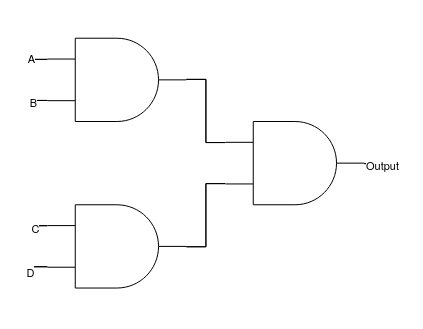
\includegraphics[scale=0.5]{figures/Andgates.png}
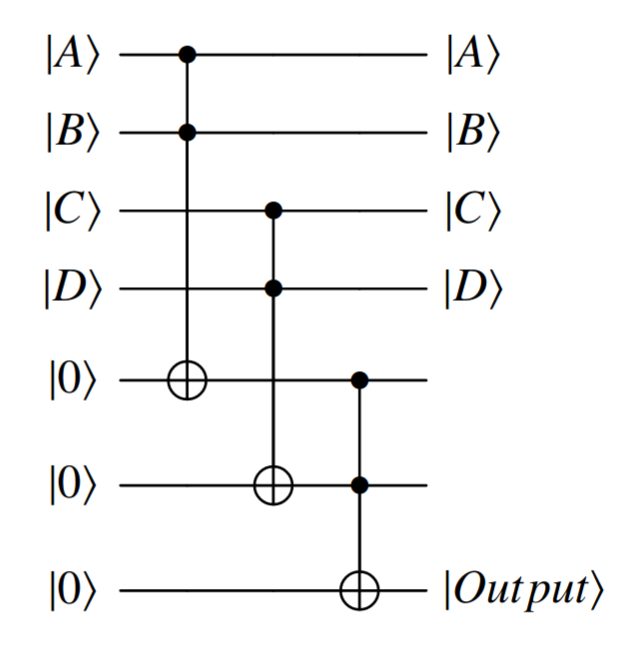
\includegraphics[scale=0.2]{figures/Qcircuit.png}
\caption{Example of how a classical circuit would be translated into a quantum circuit. The classical ${\tt AND}$ gates are replaced by the Toffoli gate.}
\end{center}
\end{figure}

There are many ways to achieve the creation and implementation of quantum gates. Some of them will be discussed in more detail in Section 2.2.6. Let us see in general how a quantum gate could be implemented. To apply a quantum gate to the qubit means to operate on a quantum state with a unitary operator. The time evolution operator discussed priorly is unitary by definition, and it acts on states according to the Schrödinger equation. The time evolution operator seems like a good candidate to be used to implement quantum gates since they share many common properties.


\subsubsection{Some important gates and universal computation}
Quantum gates are used to apply operations to qubit states. By using gates as standardized building blocks for algorithms we can restrict us to the creation of these gates. A set of gates is called universal if those gates can be used to approximate any gate to arbitrary precision. Some of the most common gates are the Pauli gates, $X, Y, Z$, which are equivalent to the Pauli matrices, $\sigma_x,\sigma_y,\sigma_z$. 
They are defined as
\begin{equation}
X \dot{=}\begin{pmatrix}
0 & 1 \\ 1 & 0
\end{pmatrix},\; 
Y\dot{=}\begin{pmatrix}
0 & -i \\ i & 0
\end{pmatrix},\; 
Z \dot{=} \begin{pmatrix}
1 & 0 \\ 0 & -1
\end{pmatrix}.
\end{equation}
It is more common to use only $X$ and $Z$ since $Y = i\,X\,Z$. The dotted equal sign,$\dot{=}$, means \textit{is represented by}. The $X$-gate is somewhat analogous to the classical {\tt NOT}-gate,  
with the effect that is swaps the input qubits, 
$$\begin{cases} X\ket{0} = \ket{1}\\
X\ket{1} = \ket{0}
\end{cases}.$$
The Z-gate introduces a phase-flip between the inputs, it does nothing to $\ket{0}$ and reverses the sign of $\ket{1}$, $$\begin{cases} Z\ket{0} = \ket{0}\\
Z\ket{1} = -\ket{1}
\end{cases}.$$ 
Superposition is one of the key aspects that make QC able to surpass classical algorithms. The Hadamard gate, $H$, creates a superimposed quantum state, and is widely used all over QC. The gate is defined as
\begin{equation}
H \dot{=} \dfrac{1}{\sqrt{2}}\begin{pmatrix}
1 & 1 \\ 1 & -1
\end{pmatrix}.
\end{equation}
Another noteworthy property is that $H$ is its own inverse, $HH = \mathbf{1}$, so it can be used both to open and close superposition. More explicitly, the gate effect is,
\begin{equation}
\begin{cases}
H\ket{0} = \dfrac{1}{\sqrt{2}}(\ket{0} + \ket{1})
\\
H\ket{1} = \dfrac{1}{\sqrt{2}}(\ket{0} - \ket{1})
\end{cases}
\text{and}\hspace{4mm}
\begin{cases}
H\dfrac{1}{\sqrt{2}}(\ket{0} + \ket{1}) = \ket{0}
\\
H\dfrac{1}{\sqrt{2}}(\ket{0} - \ket{1}) = \ket{1}
\end{cases}.
\end{equation}
Many well known quantum algorithms make heavy use of this operator \cite{Grover,shor}, making it is essential to QC.
The concept of the phase flip, $Z$, can be extended to a phase shift of any arbitrary angle. The gate is denoted by $P(\phi)$ or sometimes simply $\phi$. It is defined as 
\begin{equation}
P(\phi) \dot{=} \begin{pmatrix}
1 & 0 \\
0 & e^{i\phi}
\end{pmatrix}.
\end{equation}
In terms of the phase shift gate, $Z$ reduces to the case $P(\pi) = Z$. Some other notable cases of the phase shift are the $T$ and $S$ gates, defined by
\begin{equation}
T = P({\pi/4}) \dot{=} \begin{pmatrix}
1 & 0 \\ 0 & e^{i\pi/4}
\end{pmatrix},\, S = T^2 = P({\pi/2}) \dot{=} \begin{pmatrix}
1 & 0 \\ 0 & e^{i\pi/2}
\end{pmatrix}.
\end{equation}

All gates so far are single-qubit gates. To achieve full universality it turns out that two-qubit gates are enough. The two-qubit gate most commonly used is the ${\tt CNOT}$, which stands for controlled not, the effect is defined as ${\tt CNOT}\ket{x,y} = \ket{x,x\oplus y}$, where $\oplus$ denotes addition modulo 2. The gate takes two inputs, the control, and the target. If the control is $\ket{1}$ then a ${\tt NOT}$ is applied to the target $\ket{y} \mapsto X\ket{y}$, otherwise the gate leaves the inputs unchanged.



\subsubsection{Qudit generalizations}
Inherently there is nothing special about bits and binary logic, the same goes for qubits.  A qudit is a general name for a  $d$-dimensional computational element. The special case of $d = 3$ is called a \textit{qutrit}, $d = 4$ a \textit{ququart} and so on. A larger computational basis could even prove to be better. The information content per unit is higher, $N$ qubits can be reduced down to $\dfrac{N}{\log_2(d)}$ qudits  \cite{info_qudit}. The qutrit has a reduction factor of $\sim 0.64$, the ququart $0.5$, with less returns for higher dimensions. Due to more information per unit, fewer operations are required to build quantum gates, minimizing the loss of accuracy from operations. The drawback is the increased complexity in the schemes for physical implementation which could come with increased errors. There are already many promising results using qudits \cite{qutrit1,qudit2,qudit3}, and many more are discussed in \cite{qudit}. The interesting question is if the benefits of qudits can outweigh the extra costs associated with more complex structures.

In the following section, let the dimension $d$ be any integer such that $d \geq 3$. Some generalized qudits gates are defined and discussed. The definitions used are the same used in \cite{qudit}.
The effect of ${\tt NOT}$ is ambiguous when the number of basis states are more than 2. So instead of viewing it as ${\tt NOT}$, it can be thought of as a cyclic permutation of the states $\ket{0},\ket{1}$. The higher dimensional correspondence of $X$ is defined as
\begin{equation}
X_d = \begin{pmatrix}
0 & 0 & \dots & 0 & 1\\
1 & 0 & \dots & 0 & 0\\
0 & 1 & \dots & 0 & 0\\
\vdots & \vdots &\ddots& \vdots&\vdots\\
0 & 0& \dots & 1 & 0
\end{pmatrix}.
\end{equation}
The effect works as a permutation of basis states, for $d = 3$, the effect would be $\ket{0} \xrightarrow{X_3} \ket{1} \xrightarrow{X_3} \ket{2} \xrightarrow{X_3} \ket{0}$.
The higher dimensional $Z$-gate $Z_d$ is defined as 
\begin{equation}
Z_d = \begin{pmatrix}
1 & 0 & 0 & \dots & 0 \\
0 & \omega & 0 &\dots & 0\\
0 & 0 & \omega^2&\dots & 0 \\
\vdots & \vdots&\vdots&\ddots& 0\\
0 & 0& 0&\dots  & \omega^{d-1}
\end{pmatrix}
\end{equation}
with $\omega = e^{2\pi i/d}$ being the $d$th root of unity. It shifts the different basis states a certain amount from each other. The generalized version of the Hadamard gate for qudits, $H_d$, is more convenient to define in Dirac notation, the effect is 
\begin{equation}
H_d = \dfrac{1}{\sqrt{d}}\sum_{i=0}^{d-1} \omega^{i\,j}\ket{i}\bra{j},\; j\in \{0,1,2, \dots, d-1\}
\end{equation}
where $\omega$ again denotes the $d$th root of unity.

Last let us define the generalized qudit $T$-gate, now $d$ is restricted to prime numbers, such that $T_d$ is only defined for prime number dimensions \cite{8gate}. 
The gate is defined by
\begin{equation}
T_d = \sum_{k=0}^{d-1} \omega^{\nu_k}\ket{k}\bra{k}
\end{equation}
with $\omega$ being the $d$th root of unity. The exponent $\nu_k$ can be recursively defined with $\gamma',z',\varepsilon' \in \mathbb{Z}_d$ restricted by
\begin{equation}
\begin{cases}
\nu_0 = 0\\
\nu_{k+1} = \nu_k + k(2^{-1}\gamma'k + z') + 2^{-1}z' + \varepsilon'.
\end{cases}
\end{equation} 
In this report, $T_3$ with $z' = 1, \gamma' = 2$ and $\varepsilon' = 0$ will be implemented. This gate reads 
\begin{equation}
T_3 = \begin{pmatrix}
1 & 0 & 0\\
0 & e^{2\pi i/9}& 0 \\
0 & 0 & e^{-2\pi i /9}
\end{pmatrix}.
\end{equation}

Likewise, as for qubits, single qudit universality can be obtained by a combination of some of these gates. The universal set of gates for the qudit is the generalization of the universal set for the qubit, $\{T_d, H_d\}$. Since the $T_d$-gate is only defined in prime number dimensions universality cannot be obtained in this manner in non-prime dimensions.




\subsubsection{Dark states, bright states and dark paths}
Pod-like systems are an important type of quantum system and are used frequently in geometric QC. A pod-like system refers to a type of system with most commonly, but not limited to, one excited state coupled to a number of ground states, states can only be transformed into states to which they are coupled, with no additional coupling between the ground states. This section defines some common terms and concepts that will be used in the later sections.

For a given Hamiltonian, $H$, the eigenvalues correspond to the energies of the system. Let us denote a state with zero energy as $\ket{d}$. It holds then that
\begin{equation}
H\ket{d} = 0\ket{d},
\end{equation}
which is to say that $\ket{d}$ is an eigenstate with eigenvalue $0$. We say that $\ket{d}$ is a \textbf{dark state} of $H$. $\ket{d}$ forms a 1-dimensional dark subspace, and in general the dimension of the full dark subspace is equal to the number of dark states. All states in the dark sub-space will have $0$ energy. Furthermore we say that any state $\ket{b}$ such that 
\begin{equation}
\bra{d_k}\ket{b} = 0
\end{equation}
is called a \textbf{bright state} provided it is orthogonal to all dark states of the systems, $\ket{d_k}$. A pod-like system with $n$ ground states and $m$ excited states will have $n-m$ dark states and $m$ bright states \cite{lambda}.
The Hamiltonian can be rewritten in the \textit{dark-bright} basis (Morris-Shore basis), an equivalent basis spanned by the bright and dark states. Since the dark states are all individually decoupled from the Hamiltonian this new basis can be further split into two subspaces, one containing the bright states and one containing the dark states. This reduction can be useful since it simplifies the dynamics of the system. 
The dynamics is determined by to the Hamiltonian of the system. The part of the time evolution affected by the Hamiltonian, for some ordered basis, is $H_{nm}(t) = \bra{n}H(t)\ket{m}$. In the adiabatic case if the system starts in the dark subspace, it will remain there through-out the evolution and the dynamical phase will have no contribution to the total time evolution. In a non-adiabatic case the time evolution of the states is more complex due to the mixing of the eigenstates. So by constructing a Hamiltonian such that all $H_{nm}$ elements are zero there will be no dynamical contribution. Another way to assure no dynamical phase is to evolve the system along a \textbf{dark path}, a dark path is a state $\ket{D(t)}$ such that 
\begin{equation}
\bra{D(t)}H(t)\ket{D(t)} = 0, \, \forall t\in[0,T].
\end{equation}
this means that the expectation value of the energy will always be $0$, and thus all elements of the dynamical phase will be $0$. The dark state in itself satisfy this condition and such is a trivial dark path. By explicitly finding a dark path the parameters in the Hamiltonian can be reverse-engineered from the Schrödinger equation, enabling more complex Hamiltonians that can fulfill the NHQC criteria.


\subsubsection{Geometric quantum computation}
By making use of the geometric phases in periodic quantum systems schemes that perform computations are obtainable. Holonomic Quantum Computation (HQC) makes use of holonomies, which is to what extent parallel transport around some closed-loop fails to preserve the transported data. In the case of Quantum mechanics this means that a state, gains an additional geometric phase alongside the dynamical phase. This concept was first introduced by M.V. Berry \cite{berry} and thus the phase is usually referred to as the Berry phase, but is more generally called the geometric phase since the phase arises from the geometry rather than the dynamics of the system. The geometric phase exists also in non-adiabatic and non-abelian contexts, which gives room for more complex structures \cite{anandan1, anandan2, zee}. 
In the adiabatic setting universal computation can be achieved through holonomies by transporting a set of control parameters along a loop(s) in a suitable space \cite{HQC}. 

For an arbitrary periodic state $\ket{\psi(T)}$ after one period $T$, the Schrödinger equation (\ref{eq:schro}) has a solution on the form 
\begin{equation}
\label{eq:gen_sol}
\ket{\psi(T)} = U(T,0)\ket{\psi(0)}
\end{equation}
where in addition to the ordinary dynamical phase discussed earlier a geometric phase is present. For an ordered time dependent basis $\ket{1(t)}, \ket{2(t)},\dots, \ket{N(t)}$ a quantum state can be expanded into 
\begin{equation}
\ket{\psi} = \sum_{n = 1}^N c_{:n}\ket{n}
\end{equation}
taking the time derivative gives
\begin{equation}
\label{eq:td1}
\dot{\ket{\psi}} = \sum_{n = 1}^N \left[\dot{c}_{:n}\ket{n} + c_{:n}\dot{\ket{n}} \right].
\end{equation}
By the Schrödinger equation $\dot{\ket{\psi}}$ is equivalent to
\begin{equation}
\label{eq:td2}
\dot{\ket{\psi}} = -i\,H\ket{\psi} = -i\sum_{n = 1}^N c_{:n}H\ket{n}
\end{equation}
equating (\ref{eq:td1}) and (\ref{eq:td2}) and taking the inner product with $\bra{m}$ one obtains the expression
\begin{equation}
-i c_{mn}\bra{m}H\ket{n} = \dot{c}_{mn} + \sum_{n = 1}^N c_{mn} \bra{m}\ket{\dot{n}}
\end{equation}
re-organizing the terms  
\begin{equation}
\dot{c}_{mn} = -i\left[c_{mn}\bra{m}H\ket{n} - \sum_{n = 1}^N i c_{mn} \bra{m}\ket{\dot{n}} \right].
\end{equation}
In matrix form this can be written as 
\begin{equation}
\dot{\mathbf{C}} = i\left[\mathbf{A} - \mathbf{H} \right]\mathbf{C},
\end{equation}
where $\mathbf{A}_{mn}(t) = i\bra{m(t)}\pdv{}{t}\ket{n(t)}$ and
$\mathbf{H}_{mn}(t) = \bra{m(t)}\mathbf{H}(t)\ket{n(t)}$. The formal solution is 
\begin{equation}
\label{eq:unitary}
C = U(T,0) = \mathcal{T}\exp\left(i\int_{0}^{T} \underbrace{\mathbf{A}(t)}_{\text{Geometric}} - \underbrace{\mathbf{H}(t)}_{\text{Dynamic}}\,dt\right)
\end{equation}
If a system is periodic and a scheme can be constructed such that the dynamical phase will have no contribution to the time evolution during a full period, the period can also be described as a loop, $C$, in parameter space. So for a period the operator can be written as
\begin{equation}
U(T,0) = \mathcal{T}\exp\left(i\int_{0}^{T}\mathbf{A}(t)\,dt\right) = \mathcal{P}\exp\left(i\oint_{C}\mathbf{A}(s)\,ds\right) = U(C),
\end{equation}
where $\mathcal{P}$ denotes path-ordering. This is the Wilczek-Zee holonomy which can be used to achieve geometric quantum computation. 

In the adiabatic case it is enough for the system to start in a dark sub-space since the states will evolve without mixing. Thus the energy associated with the Hamiltonian will be zero through-out the whole time evolution. Therefore it is possible to construct unitaries by pure geometric means by starting in the correct state \cite{adiabatensatz,AHQC}.

\begin{figure}[H]
\begin{center}
    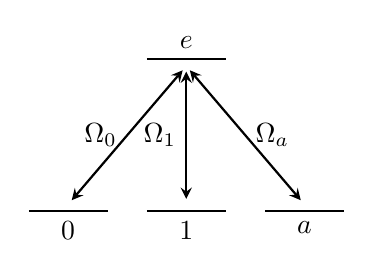
\begin{tikzpicture}[
      scale=0.5,
      level/.style={thick},
      virtual/.style={thick,densely dashed},
      trans/.style={thick,<->,shorten >=2pt,shorten <=2pt,>=stealth},
      arrow/.style={thick,->,shorten >=2pt,shorten <=2pt,>=stealth},
      classical/.style={thin,double,<->,shorten >=4pt,shorten <=4pt,>=stealth}]
      
    % Excited
    \draw[level] (7cm,0em) -- (9cm,0em) node[midway,above] {$\ket{e}$};
	% Ground states
    \draw[level] (4cm,-11em) -- (6cm,-11em) node[midway,below] {$\ket{0}$};
    \draw[level] (7cm,-11em) -- (9cm,-11em) node[midway,below] {$\ket{1}$};
    \draw[level] (10cm,-11em) -- (12cm,-11em) node[midway,below] {$\ket{a}$};
    % e_1
    % Draw the transitions.
    \draw[trans] (8cm,-0.5em) -- (5cm,-10.5em) node[midway,left]  {$\Omega_0$};
    \draw[trans] (8cm,-0.5em) -- (8cm,-10.5em) node[midway,left] {\hspace{2mm}$\Omega_1$};
    \draw[trans] (8cm,-0.5em) -- (11cm,-10.5em) node[midway,right] {$\Omega_a$};
    
    \end{tikzpicture}    
    \caption{System described by the Hamiltonian in Equation \ref{eq:AHQCH}.} 
     \label{fig:HamAH}
    \end{center}

\end{figure}
A well known result that makes use of the Wilczek-Zee holonomy to obtain universal computation presented by L.M. Duan in \cite{AHQC}. By using a tripod system defined by the Hamiltonian
\begin{equation}
\label{eq:AHQCH}
H = \ket{e}[\Omega_0\bra{0} + \Omega_1\bra{1} + \Omega_a\bra{a}] + \;\text{h.c},
\end{equation}
the system is shown in Figure \ref{fig:HamAH}. By manipulating the parameters and the coupling strengths this Hamiltonian can be used to create a set of universal gates; $U_1 = e^{i\phi_1\ket{1}\bra{1}} = \begin{pmatrix}
1 & 0\\
0 & e^{i\phi_1}
\end{pmatrix}, U_2 =  e^{i\phi_2\sigma_y} = R_y(\phi_2), U_3 =  e^{i\phi_3\ket{11}\bra{11}}$.
Let us calculate $U_1$, which is a phase gate, to see how this is obtained. First the parameters are chosen as $\Omega_0 = 0,\,\Omega_1 = -\Omega\sin\frac{\theta}{2}e^{i\varphi},\, \Omega_a = \Omega\cos\frac{\theta}{2}$. The Hamiltonian in this case is 
\begin{equation}
H  = \ket{e}\left[-\Omega\sin\frac{\theta}{2}e^{i\varphi}\bra{1} + \Omega\cos\frac{\theta}{2}\bra{a}\right] + \;\text{h.c},
\end{equation}
where +\;h.c is read as Hermitian conjugate, thus $A +\;\text{h.c} = A + A^\dagger$. Then find a dark state $\ket{d}$ to the Hamiltonian such that $H\ket{d} = 0$. In this state the energy will be zero and by evolving the system adiabatically the energy will remain zero. The dark state is $\ket{d} = \cos\frac{\theta}{2}\ket{1} + \sin\frac{\theta}{2}e^{i\varphi}\ket{a}$. By starting in the state $\theta = 0$, then $\ket{d} = \ket{1}$ and evolving the new control parameters in a closed loop in parameter space we find that the holonomy is independent of the path and $U_1 = e^{i\phi_1\ket{1}\bra{1}}$ where $\phi_1$ is the enclosed solid angle obtained by the vector $(\theta,\varphi)$ during the evolution, $\phi_1 = \oint \sin\theta\; d\theta \;d\varphi$. The other single-qubit gate $U_2$ is obtained in a similar way and $U_3$ requires some extra work by using detuning to create a two-qubit gate.



Due to the long runtimes associated with adiabatic evolution the state is prone to errors and decoherence from outside factors \cite{NHQC}. As a consequence, in the non-adiabatic case (NHQC), it would be possible to construct faster and more robust gates. Since the states are mixing some other way to control $U$ must be engineered. By removing the dependence on the dynamics of the system, the period time, and the energies in the time evolution, that is by some other mean ensure that 
\begin{equation}
\bra{m(t)}H(t)\ket{n(t)} = 0,\,\forall m,n, t\in[0,T]
\end{equation} 
holds. This means all terms in the dynamical phase in (\ref{eq:unitary}) are zero.
This is possible given that there exist a two-pulse non commuting loop, $C = C_1 \cup C_2$, \cite{NHQC,sLoop}, 
then the unitary will be reduced to 
\begin{equation}
U(T,0) = \sum_{n,m = 1}^{N} U_{nm}\ket{n(0)}\bra{m(0)}
\end{equation}
and can be used to perform any arbitrary quantum gate on the computational space.

The idea of NHQC can be extended by instead of explicitly constructing a Hamiltonian with non-dynamical interaction, one can construct explicit dark paths through parameter space that satisfy the NHQC criteria. In \cite{darkpath} a qubit scheme is constructed and experimentally implemented in a trapped $^{171}Yb^{+}$ ion, using a dark path. They conclude that arbitrary NHQC gates can be constructed with better robustness. We will build upon the scheme presented and create an explicit qutrit example, then speculate how it can be generalized to higher dimensions.

\subsection{Research Questions}

Holonomic quantum compuatation is an instresting research area due to the potential of high resilience to errors arising from constructing gates from global holonomies. Furthermore non-adiabatic implementations are desirable since shorter run times can decrease decoherance during the time evolution of systems and thus make even sturdies gates. There has already been several holonomic implementations of qubits, both adiabatic and non-adiabatic \cite{HQC, NHQC} but here we aim at implementing higher dimensional qudits in a non-adiabatic holonomic setting. 

\begin{itemize}
\item \textbf{Research question 1: How does the NHQC qubit implementation using dark path generalize to higher computational elements?} We are insterested to see how the implementation of the qubit in \cite{darkpath} could be generalized for qudits. This is achieved by finding a way to extend the quantum system in such a way that a qudit can be encoded. 

\item \textbf{Researcg question 2: Is gate robustness still high for qudits?} The upside of NHQC is the high error resilience in the quantum gates. We want to study if similar behavior is present in higher dimensions. We also test ways to improve robustness by the inclusion of an auxiliary state.



\end{itemize}






